\chapter{Background and literature review}\label{chap:background}
\section{Background}

\subsection{Car Modeling}
\subsubsection{Quarter Car Model}
The quarter car model is a simplified vehicle dynamics model representing one wheel, the suspension system, and one-quarter of the vehicle body mass. It is mainly used to study vertical ride dynamics, suspension performance, and vibration response while maintaining low computational complexity.
\begin{figure}[H]
    \centering
    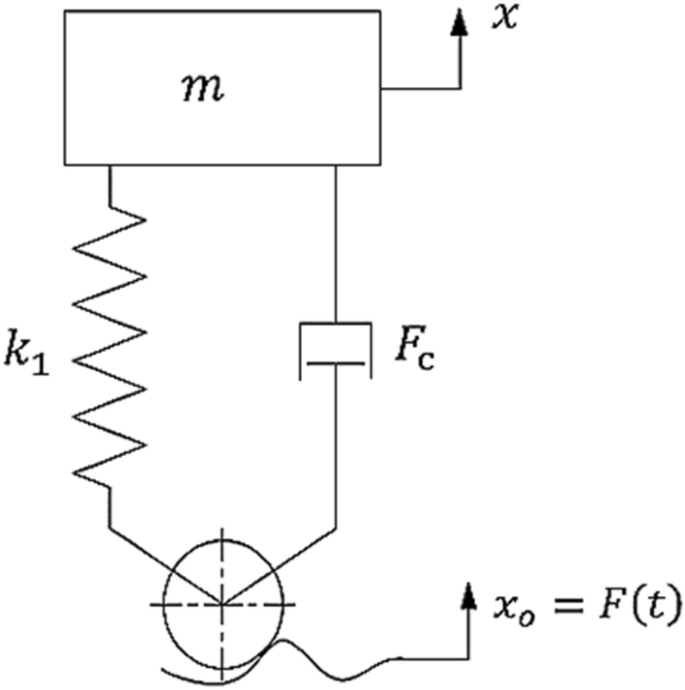
\includegraphics[width=0.5\linewidth]{Thesis Pictures/qcm.png}
    \caption{Quarter car model}
    \label{fig:qcm}
\end{figure}
\subsubsection{Half Car Model}
The half car model represents either the front and rear sections or the left and right sides of a vehicle. It considers additional motions such as pitch or roll, allowing more accurate analysis of braking, acceleration, and load transfer effects compared to the quarter car model.
\begin{figure}[H]
    \centering
    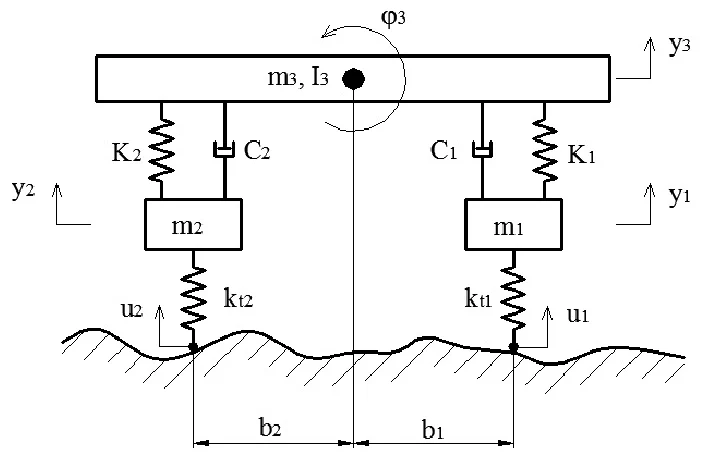
\includegraphics[width=0.5\linewidth]{Thesis Pictures/HCM (1).png}
    \caption{Half car model}
    \label{fig:hcm}
\end{figure}
\subsubsection{Full Car Model}
The full car model represents the complete vehicle system, including all four wheels, suspension components, and body motions. It accounts for vertical, pitch, and roll dynamics simultaneously, providing the most comprehensive analysis of vehicle stability, ride comfort, and handling performance.
\begin{figure}[H]
    \centering
    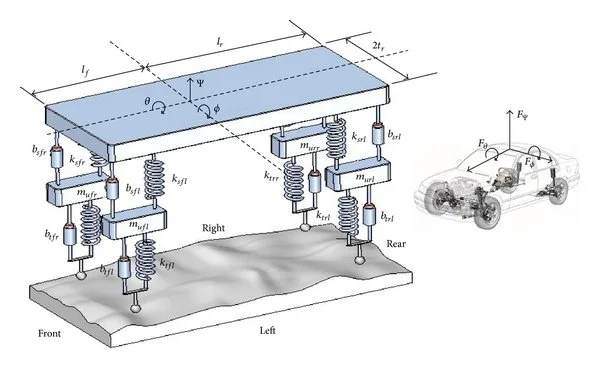
\includegraphics[width=0.5\linewidth]{Thesis Pictures/fcm1.png}
    \caption{Full car model}
    \label{fig:fcm}
\end{figure}
\subsection{Dampers}
\subsubsection{Hydraulic}
Hydraulic dampers dissipate vibration energy through the controlled flow of hydraulic fluid inside the damper. The resistance generated by the fluid motion produces the damping force required to reduce suspension oscillations. They are widely used due to their simplicity, reliability, and low cost.
\subsubsection{Electromagnetic}
Electromagnetic dampers use electromagnetic induction to generate damping forces from the relative motion between magnetic and conductive components. In regenerative suspension systems, they can convert part of the vibration energy into electrical energy, improving overall vehicle energy efficiency while maintaining ride stability.
\subsubsection{Magnetorheological}
Magnetorheological dampers use a special fluid containing magnetic particles whose viscosity changes when exposed to a magnetic field. By controlling the magnetic field strength, the damping force can be adjusted in real time, allowing improved ride comfort, adaptability, and vehicle handling performance.

\subsection{Force Control}
\subsubsection{Skyhook}
Skyhook control is a semi-active suspension control strategy designed to improve ride comfort by reducing vehicle body motion. It simulates a virtual damper connected between the vehicle body and an imaginary fixed point in the sky, helping minimize vertical body acceleration and vibrations.
\subsubsection{Groundhook}
Groundhook control focuses on improving road holding and tire contact stability by minimizing wheel and unsprung mass motion. It behaves as if a virtual damper is connected between the wheel assembly and the ground, enhancing tire-road contact and vehicle handling performance.
\subsubsection{Hybrid Skyhook-Groundhook}
Hybrid skyhook-groundhook control combines the advantages of both skyhook and groundhook strategies. It aims to achieve a balance between ride comfort and road holding by simultaneously reducing body vibrations and maintaining stable tire-road contact.
\begin{figure}
    \centering
    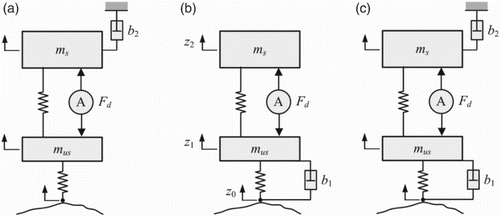
\includegraphics[width=0.5\linewidth]{Thesis Pictures/Hook Controls (1).png}
    \caption{(a) Skyhook control (b) Groundhook control \newline (c) Hybrid skyhook-groundhook control}
    \label{fig:hook_controls}
\end{figure}
\subsubsection{Energy-Aware}
Energy-aware control strategies consider both suspension performance and energy consumption or regeneration. In regenerative suspension systems, this approach optimizes damping behavior while maximizing the amount of electrical energy harvested from suspension vibrations.
\subsubsection{MPC}
Model Predictive Control (MPC) is an advanced control strategy that predicts future system behavior using a mathematical model of the vehicle. It optimizes suspension control inputs over a prediction horizon while considering system constraints, enabling improved ride comfort, handling stability, and energy efficiency.

\subsection{Current Control}
\subsubsection{PI}
PI current control is a widely used control method for regulating current in electrical systems and actuators. The proportional term responds to the instantaneous current error, while the integral term eliminates steady-state error over time. PI controllers are simple, computationally efficient, and effective for maintaining stable current tracking in electromagnetic actuator applications.
\subsubsection{SMC}
Sliding Mode Control (SMC) is a nonlinear robust control technique used to achieve accurate current regulation under system uncertainties and disturbances. It drives the system states toward a predefined sliding surface and maintains them on it despite parameter variations or external disturbances. In current control applications, SMC offers fast dynamic response, high robustness, and improved stability compared to conventional linear controllers, although it may introduce chattering effects if not properly designed.

\subsection{Power Converters}
\subsubsection{Buck}
A buck converter is a DC-DC power converter that steps down the input voltage to a lower output voltage. It operates by switching and energy storage in an inductor, providing high efficiency and smooth output when properly filtered. It is commonly used where a regulated lower voltage is required from a higher supply.
\subsubsection{Boost}
A boost converter is a DC-DC power converter that steps up the input voltage to a higher output voltage. It stores energy in an inductor during the switching phase and releases it at a higher voltage level, enabling voltage amplification with relatively high efficiency.
\begin{figure}[H]
    \centering
    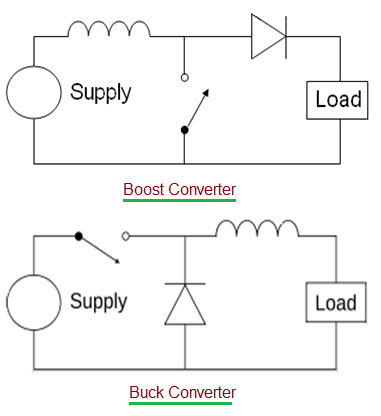
\includegraphics[width=0.5\linewidth]{Thesis Pictures/converters.png}
    \caption{Buck and boost converter topologies}
    \label{fig:converters}
\end{figure}
\subsubsection{Uni-directional Buck-Boost}
A unidirectional buck-boost converter can either step up or step down voltage, but power flows in only one direction (from source to load). It is used when bidirectional energy flow is not required, such as regulated power supplies or fixed-direction energy harvesting systems.
\subsubsection{Bi-directional Buck-Boost}
A bidirectional buck-boost converter allows power flow in both directions and can operate in both step-up and step-down modes. It is essential in systems involving energy storage, such as batteries or regenerative systems, where energy must be exchanged between the source and storage element (e.g., regenerative suspension or electric vehicles).

\subsection{Control Strategies}
\subsubsection{Passive}
Passive suspension systems use fixed mechanical components such as springs and dampers with constant properties. They do not require external power or control input. Performance is determined at the design stage and cannot adapt to changing road or driving conditions. They are simple, reliable, and cost-effective but offer limited optimization between ride comfort and road handling.
\subsubsection{Active}
Active suspension systems use actuators to generate external forces based on control inputs. They can both add and remove energy from the system, allowing precise control of body motion, ride comfort, and tire contact. Although they provide the highest performance in terms of stability and comfort, they are more complex, expensive, and energy-intensive.
\subsubsection{Semi-Active}
Semi-active systems adjust damping characteristics in real time without actively injecting energy into the system. They typically use controllable dampers (e.g., magnetorheological or variable orifice dampers). These systems improve performance by adapting to road conditions while maintaining low power consumption and high safety since they cannot generate active forces.

  \subsection{Metrics}
  To evaluate the performance of the regenerative suspension model, we need to refer to metrics that inform us about the effectiveness of our control algorithm.
  \subsubsection{Tyre Dynamic Load}
    Tyre dynamic load refers to the variation of vertical force acting on a tire during vehicle motion due to acceleration, braking, cornering, and road disturbances. It is an important indicator of vehicle stability because tire grip is directly influenced by the applied load. Uneven or excessive dynamic load transfer between tires can reduce overall traction, negatively affecting braking performance, steering response, and cornering stability. Therefore, controlling dynamic tire loads is essential for achieving balanced handling and maintaining vehicle stability under dynamic driving conditions.  
    \subsubsection{Body Acceleration}
   Body acceleration represents the acceleration experienced by the vehicle chassis or sprung mass during motion. It is a key parameter in evaluating vehicle stability and ride comfort, as excessive body acceleration indicates increased vibrations and oscillations transmitted to the vehicle body. High longitudinal, lateral, or vertical body accelerations can negatively affect passenger comfort, handling performance, and tire-road contact stability. Therefore, minimizing undesired body acceleration through proper suspension and damping design is essential for improving both ride quality and overall vehicle dynamics.
\subsubsection{Energy Regeneration}
 Energy regeneration in the regenerative suspension system refers to the process of converting vibration energy produced by road irregularities and vehicle body motion into electrical energy using an electromagnetic damper. Instead of dissipating suspension vibrations as heat, the electromagnetic damper harvests part of the mechanical energy through electromagnetic induction and converts it into usable electrical power. This improves overall vehicle energy efficiency while simultaneously contributing to vibration damping and vehicle stability.
 \subsection{Time-Domain Performance Indices}


Time-domain performance indices are widely used in vehicle dynamics and control systems to evaluate transient and steady-state behavior under arbitrary road excitations. In active suspension systems, these indices provide direct quantitative measures of ride comfort, road holding, and energy performance without requiring frequency-domain transformations. The following metrics are used throughout this work to ensure consistent comparison across all controllers and road scenarios.


\subsubsection{Root Mean Square (RMS) Body Acceleration}

The root mean square (RMS) of body acceleration is defined as:
\begin{equation}
a_{\mathrm{RMS}} = \sqrt{\frac{1}{T} \int_0^T a^2(t)\,dt}
\end{equation}

This metric represents the effective magnitude of the vibration experienced by the vehicle chassis over the simulation horizon. It is commonly used as a primary indicator of ride comfort, since it correlates with the overall severity of sustained oscillations. Higher RMS values correspond to poorer ride comfort.

\subsubsection{Standard Deviation of Body Acceleration}

The standard deviation is defined as:
\begin{equation}
\sigma_a = \sqrt{\frac{1}{T} \int_0^T \left(a(t) - \mu_a\right)^2 dt}
\end{equation}

where $\mu_a$ is the mean acceleration over the simulation interval. This metric quantifies the variability of the acceleration signal around its mean value and is therefore used to isolate oscillatory behavior from any steady bias. When the mean is negligible, the standard deviation approaches the RMS value.

\subsubsection{Peak Body Acceleration}

The peak acceleration is defined as:
\begin{equation}
a_{\mathrm{peak}} = \max |a(t)|
\end{equation}

This metric captures the maximum instantaneous chassis acceleration and is used to evaluate worst-case transient comfort conditions, such as impacts or resonant excitations.

\subsubsection{Vibration Dose Value (VDV)}

The vibration dose value is defined as:
\begin{equation}
VDV = \left( \int_0^T a^4(t)\,dt \right)^{1/4}
\end{equation}

This nonlinear metric places greater emphasis on high-amplitude events and is therefore particularly sensitive to shocks and impulsive disturbances. It is commonly used as a complementary measure to RMS-based comfort evaluation.


\subsubsection{Tyre Dynamic Load Variation (RMS)}

The RMS variation of tyre normal load is defined as:
\begin{equation}
\Delta F_{z,\mathrm{RMS}} = \sqrt{\frac{1}{T} \int_0^T \left(F_z(t) - F_{z0}\right)^2 dt}
\end{equation}

where $F_{z0}$ is the static tyre load. This metric quantifies the fluctuations in tyre-road contact force and is used as a primary indicator of road holding performance. Lower values correspond to more stable tyre contact.

\subsubsection{Peak Tyre Load Variation}

The peak deviation of tyre load is defined as:
\begin{equation}
\Delta F_{z,\mathrm{peak}} = \max \left|F_z(t) - F_{z0}\right|
\end{equation}

This metric captures extreme tyre unloading or overload events, which are critical for assessing potential loss of road contact or excessive tyre stress.

\subsubsection{Road Holding Index}

The road holding index is defined as:
\begin{equation}
RHI = 1 - \frac{\Delta F_{z,\mathrm{RMS}}}{F_{z0}}
\end{equation}

This normalized metric provides a dimensionless measure of tyre contact stability, where values closer to unity indicate improved road holding performance.

\subsubsection{Peak Power}

\begin{equation}
P_{\mathrm{peak}} = \max P(t)
\end{equation}

This metric represents the maximum instantaneous power demand or generation, and is used to evaluate actuator stress and electrical system limits.

\subsubsection{Root Mean Square Power}

\begin{equation}
P_{\mathrm{RMS}} = \sqrt{\frac{1}{T} \int_0^T P^2(t)\,dt}
\end{equation}

This metric represents the effective power level over time and is used to assess sustained energy demand and thermal loading.

\subsubsection{Harvested Energy}

\begin{equation}
E_{\mathrm{harvest}} = \int_0^T \max\left(P(t), 0\right)\,dt
\end{equation}

This metric quantifies the total usable energy recovered from suspension motion, considering only positive power contributions.

\subsubsection{Total Energy Throughput}

\begin{equation}
E_{\mathrm{total}} = \int_0^T \left|P(t)\right|\,dt
\end{equation}

This metric represents the total absolute energy exchanged in the system and provides a measure of overall actuator activity regardless of energy direction.

 \section{Literature review}

 \subsection{Jin-qui et al. - 2013}
Jin-qui et al. reviews the development of energy-regenerative suspension systems as a means to improve vehicle fuel efficiency by capturing kinetic energy typically lost as heat \cite{jin2013review}. The authors evaluate various mechanical and electromagnetic configurations, identifying a critical conflict between high-efficiency energy harvesting and optimal vibration control. The study concludes that hydraulic transmission and self-powered magnetorheological (MR) dampers are the most promising designs due to their superior balance of regenerative efficiency, vibration attenuation, and mechanical reliability.

\subsection{Zhang et al. - 2022}
Zhang et al. introduces a high-power density mechanical-electrical-hydraulic (MEH) regenerative suspension designed for the kilowatt-level recovery needs of high-speed tracked vehicles \cite{zhang2023research}. The system utilizes a four-quadrant hydraulic motor-generator to convert vibration-induced hydraulic energy into electricity, achieving a conversion efficiency of 40.4\%. Simulations demonstrate that damping can be adjusted via external resistance for semi-active control, with average recovery power reaching 5.293 kW under extreme off-road conditions. The study concludes that this integrated MEH design significantly improves energy utilization and reliability compared to traditional electromechanical systems.1234

\subsection{Shi et al. - 2015}
Shi et al. introduces a semi-active energy-regenerative suspension system designed to recover vibration energy while maintaining vehicle ride comfort and reducing the costs associated with traditional active systems \cite{Shi_2015}. The system features a unique energy-regenerative damper that integrates a tubular permanent-magnet linear motor with a three-level adjustable hydraulic shock absorber. A dual-loop controller manages the system: an external fuzzy controller determines the required damping force, while an inner loop regulates the motor's electromagnetic damping via a DC-DC converter and adjusts the shock absorber's base damping.
\begin{figure}[H]
    \centering
    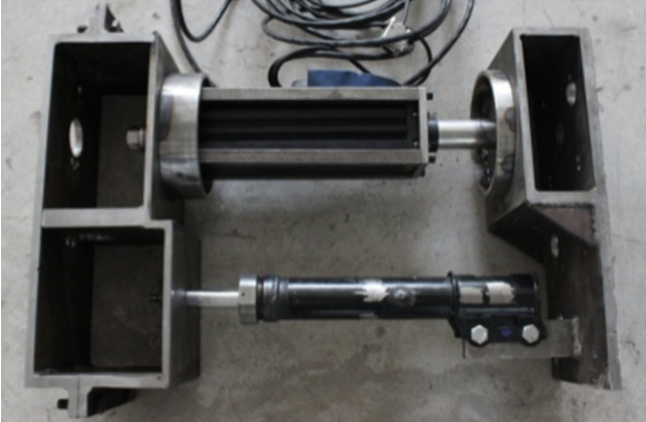
\includegraphics[width=0.5\linewidth]{Thesis Pictures/shi14.png}
    \caption{Regenerative suspension test rig}
    \label{fig:shi_rig}
\end{figure}
\subsection{Huang - 2016}
Huang develops an energy-regenerative vehicle suspension system designed to capture waste energy from road-induced vibrations while simultaneously providing dynamic vibration control \cite{huang2016energy}. The research introduces a prototype featuring a rotary direct current (DC) machine coupled with a ball screw mechanism to convert translational vehicle motion into electricity. The study provides systematic optimization methodologies for both harmonic and stochastic road excitations, offering graphical guidelines to balance the inherent trade-off between ride comfort and regenerative efficiency. Furthermore, the thesis demonstrates a bandwidth enhancement technique using cubic nonlinearities from piecewise linear springs to improve energy harvesting under varying frequencies. The study concludes that a self-powered regenerative Skyhook control strategy can successfully operate using only self-generated energy, outperforming traditional semi-active methods without requiring external power.

\subsection{Algethami - 2017}
Algethami investigates the development of a regenerative suspension system using a 2-DOF quarter-car testbed to address the world's increasing energy deficit \cite{algethami2017regenerative}. The author evaluates the trade-offs between active controllers, which provide superior vibration suppression (up to 69\%) but consume significant power (8–9 W), and regenerative designs that save energy while damping. The study identifies the symmetrical-bridgeless boost converter (SBBC) as an ideal interface due to its minimal components and ability to maintain a high power factor by keeping current and voltage in phase. The thesis concludes that while the experimental regenerative system achieved modest vibration reduction (22–24\%), it successfully demonstrates the potential to recycle power that is traditionally lost as heat, suggesting that future improvements in electromagnetic damper efficiency could lead to more economical and effective hybrid suspension systems.1234

 \subsection{Alrefaie et al. - 2022}
  Alrefaie et al. uses a semi-active neuro-fuzzy controlled magnetorheological damper to control the behavior of a full-car model \cite{alrefaie2022semi}. The neuro-fuzzy is a neural network approach to create and optimize the fuzzy rules.The results were compared against passive and PID performances on MATLAB.
  
  \subsection{Lv et al. - 2020}
  Lv et al. reviews recent developments in energy-regenerative suspension systems within the context of vehicle electrification and energy efficiency \cite{lv2020research}. Regenerative suspension systems aim to recover vibrational energy and convert it into electrical power for reuse within the vehicle. The study examines different energy recovery approaches reported in the literature, including hydraulic, electromagnetic, and hybrid configurations, with particular emphasis on hydraulically based systems due to their compatibility with existing suspension architectures.
  
   \subsection{Fu et al. - 2022}
   Fu et al. compared the advantages and disadvantages of the regenerative suspension technology between power generation and vehicle performance \cite{fu2023review}. This paper also discusses advancements in control methods, structures, and optimization techniques.

   \subsection{Davoudi et al. - 2006}
    Davoudi et al. presents a state-space average-value modeling approach for pulsewidth modulation (PWM) converters operating in both continuous and discontinuous conduction modes \cite{davoudi2006numerical}. The proposed methodology introduces a numerical extraction of the duty-ratio constraint and correction term using detailed circuit simulations, where these terms are expressed as nonlinear functions of the duty cycle and the average value of the fast state variables. The developed model is validated against a hardware prototype, detailed simulations, and existing models from literature.

  \subsection{Casavola et al. - 2017}
    Casavola et al. proposes a multiobjective $H_{\infty}$ control strategy that balances ride comfort,
    road handling, and suspension stroke with the conflicting objective of energy harvesting \cite{Casavola03042018}. Simulations were also done in CarSim that confirmed the feasibility of the proposed controller.
    
   \subsection{Shi et al. - 2019}
   Shi et al. used a hybrid skyhook-groundhook reference force to control a uni-directional buck-boost converter using sliding mode control \cite{shi2019research}. They integrated a decision module to simulate either buck or boost dynamics using its differential equations under continuous conduction mode. The effective bandwidth of controllable semi-active force is also calculated for different values of skyhook and groundhook damping.